% Chapter 6

\chapter{Event Plane} % Main chapter title

\section{Determination of Event Plane}
\label{sect:eventplane}

\begin{figure}[htbp!]
  \centering
    \begin{subfigure}[p]{0.6\textwidth}
    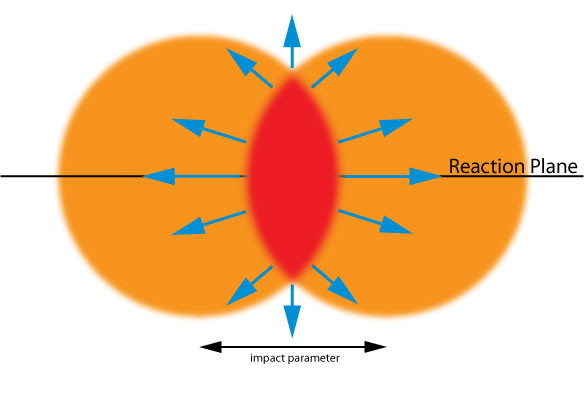
\includegraphics[width=1\textwidth]{Figures/Flow_Plane.jpg}
    \caption[Diagram showing impact parameter versus $N_spectators$ and $N_participants$]{A two-dimensional representation of the event plane. Recall the impact parameter is the distance between the two colliding ions' centers. In this illustration the orange spheres represent the ions, one is going into the page and one is coming out of and the red overlap is the matter created by the participant nucleons.
    \label{fig:cernfireball}}
    \end{subfigure}
    \begin{subfigure}[p]{0.55\textwidth}
    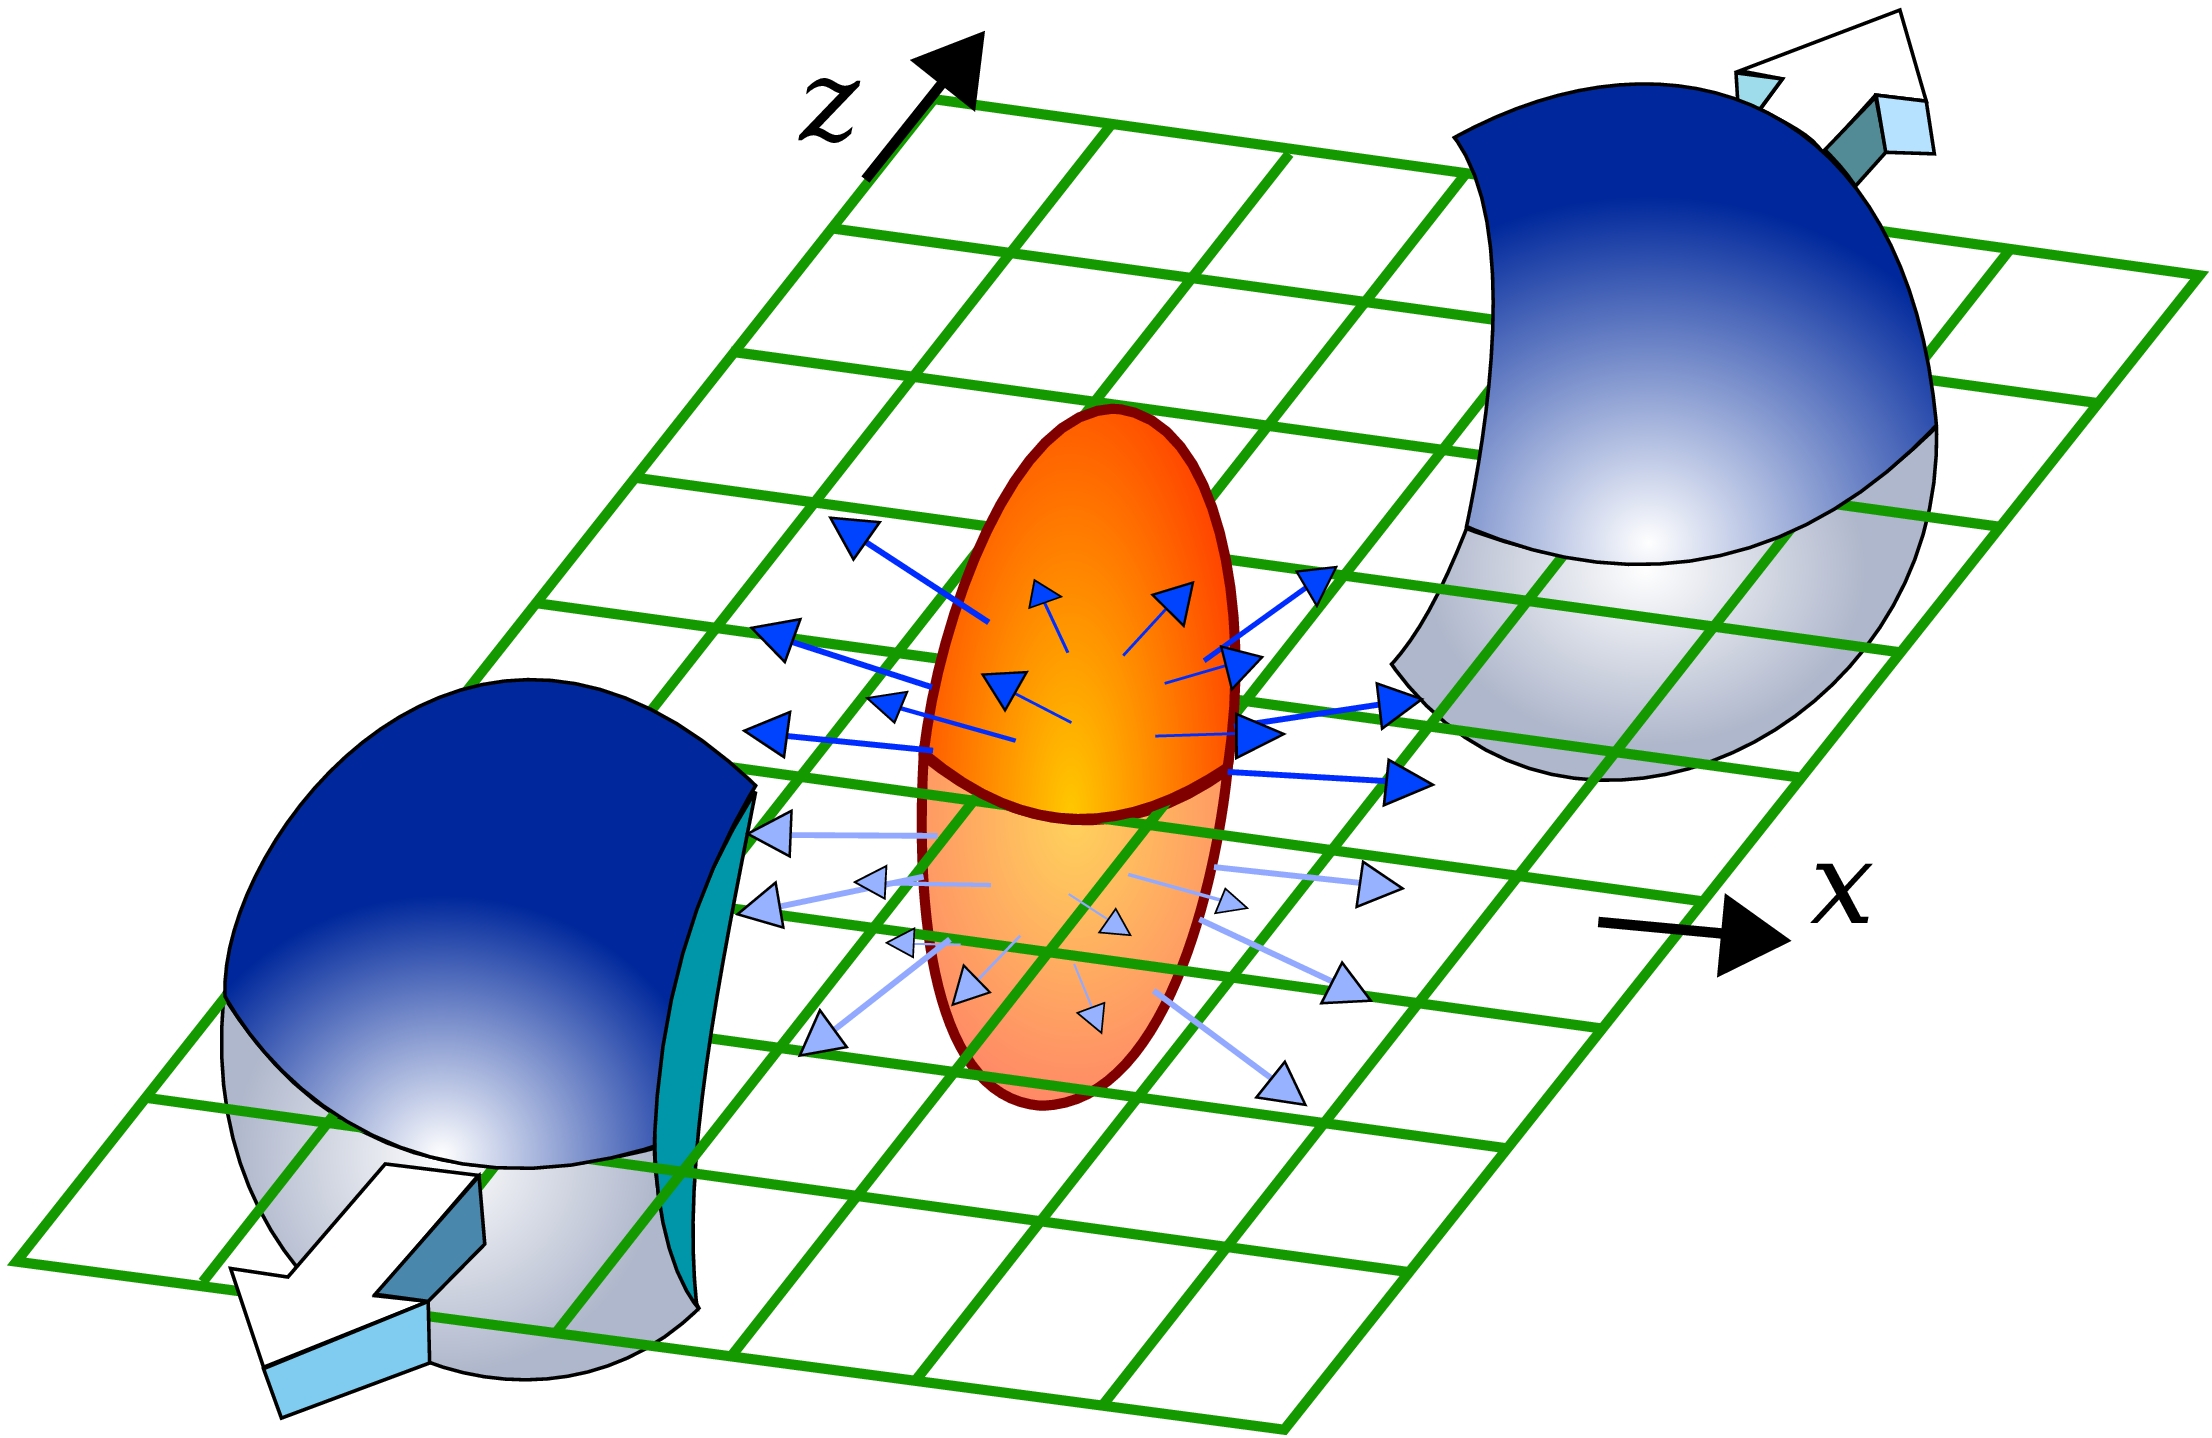
\includegraphics[width=1\textwidth]{Figures/flowcartoon.jpg}
	\caption[Central vs Peripheral collisions, geometry of initial conditions]{A three-dimensional render of the initial conditions just after a collision. The two blue spheres are the remnant spectator nucleons from the colliding ions, the orange/yellow ellipsoid is the nuclear matter created by the collision of participant nucleons. The green grid here represents the plane that bisects all three of these bodies which we call the event plane.}
    \end{subfigure}
    \rule{35em}{0.5pt}
  \caption[Illustrations of the event plane in heavy ion collisions.]{Illustrations of the event plane in heavy ion collisions.}
  \label{fig:evtpln}
\end{figure}

Pivotal to this analysis is the ability to determine an event characterization variable called the \textit{event plane}. Given the geometry of a heavy ion collision, the event plane is defined as the two-dimensional plane that bisects both ions equally through their centers as shown in Figure \ref{fig:evtpln}. Recall that the impact parameter is the distance between the two colliding ions' centers. A vector can be formed from this distance, and the plane containing both the impact parameter vector and a vector that represents the direction one of the ions is traveling down the beam axis, is the event plane\footnote{It is irrelevant which direction the impact parameter vector points and which direction we pick to point the beam axis vector, this is merely for creating a plane.}.

In practice, this plane is determined by detecting the spectator nucleons at high rapidity, or participant-created tracks at forward rapidity using detectors with full azimuthal coverage. Ideal candidates for this are the MPC, BBC, SMD, and RXNP. Particle signals would appear in the Northern detector as a cluster of hits on one side in azimuth and in the Southern detector as a cluster of hits 180$^\circ$ azimuthal degrees across (as shown in Figure \ref{fig:rxnpexpcartoon}). The event plane can therefore be constructed using the locations of these signal clusters and creating a plane that bisects them.

\begin{figure}[htbp!]
  \centering
    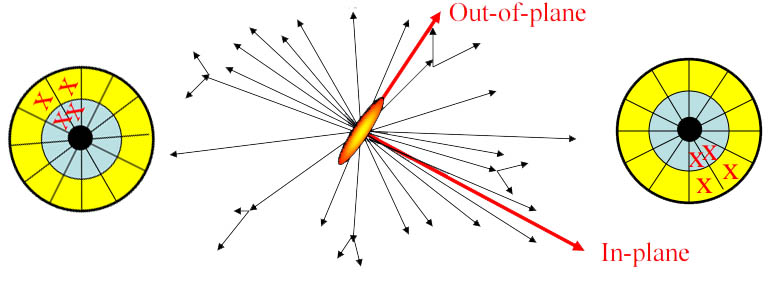
\includegraphics[width=1\textwidth]{Figures/reactionplaneexpcartoon.jpg}
    \rule{35em}{0.5pt}
  \caption[Cartoon of Event Plane determination with forward detectors]{Cartoon of Event Plane determination with forward detectors. The two target shapes represent forward detectors, in this case RXNP. The largest cluster of hits in one detector will happen along the event plane and will be correlated to a large cluster of hits in the complementing detector on the other muon arm. The orientation of these hits can then be used to reconstruct the event plane. \citep{RXNPfocus}}
  \label{fig:rxnpexpcartoon}
\end{figure}



\section{Q-vector Re-centering}
Since there is little control over the precise impact parameter and event plane orientation for each collision, the precise orientation of the ions at moment of impact cannot be controlled. As such, the event plane orientation for each event happens randomly. In order to make a meaningful flow measurement a way of aligning each of the event planes is needed. To do this, collective flow is utilized to find the plane of largest particle production along the beam axis. The weighted detector response in the x and y axes define an event plane characterizing vector called the \textit{Q-vector}. The Q-vector points in the direction of largest particle production as expected from the n-th flow harmonic. Therefore, specific event planes are determined for each flow coefficient studied, i.e. if a second order particle distribution is used to determine the Q-vector, the Q-vector characterizes the second order event plane. The BBC and SMD detect the remnants of a collision and are able to analyze their distribution in the x and y axis. This distribution is Gaussian and models the direction the Q-vector points. Shifting the x and y mean of this distribution to 0 in both axes aligns the planes for all events.

\section{Event Plane ``Flattening"}
Furthermore, because event plane orientations populate a distribution randomly, the distributions are expected to be uniform. However, the imperfections and acceptance limitations of the event plane characterizing detectors cause this distribution to be non-uniform. The process of making this distribution uniform in azimuth is called \textit{flattening}.

\begin{figure}
  \centering
    \begin{subfigure}[p]{0.4\textwidth}
    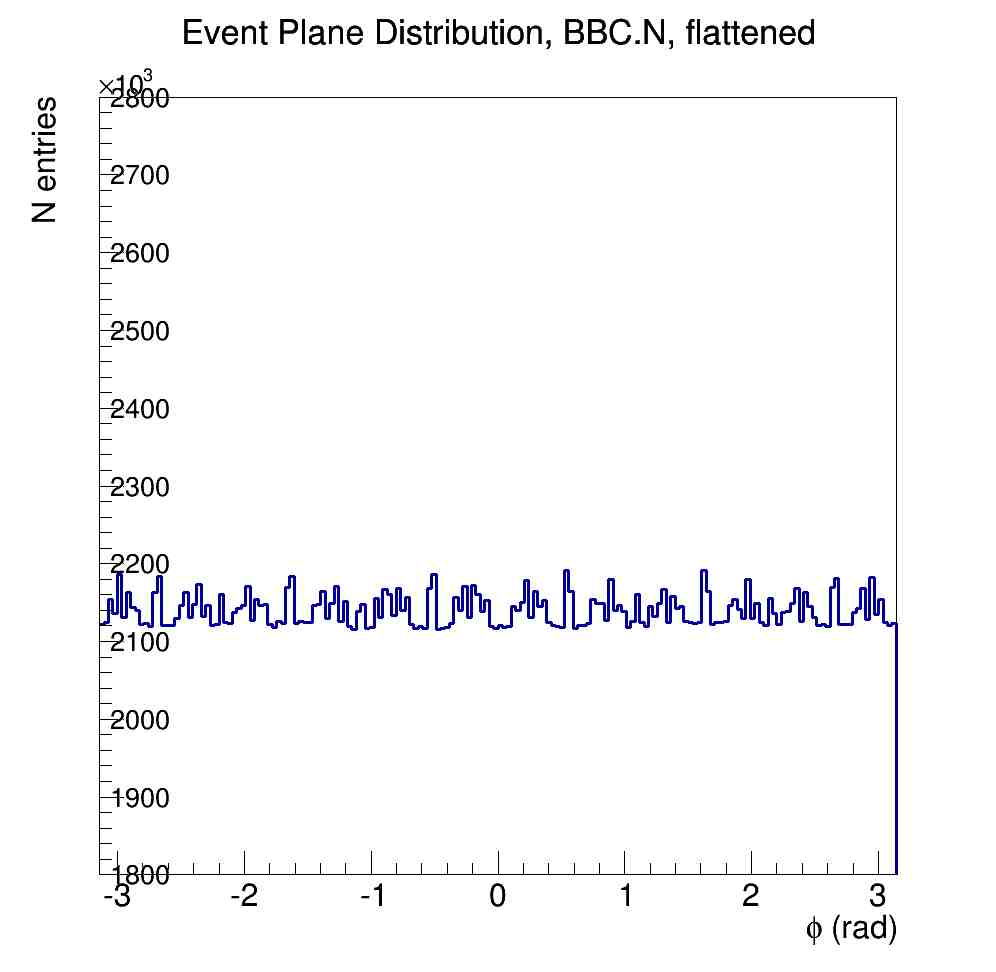
\includegraphics[width=1\textwidth]{EPflattening/flatbbcn.jpg}
    \end{subfigure}
    \begin{subfigure}[p]{0.4\textwidth}
    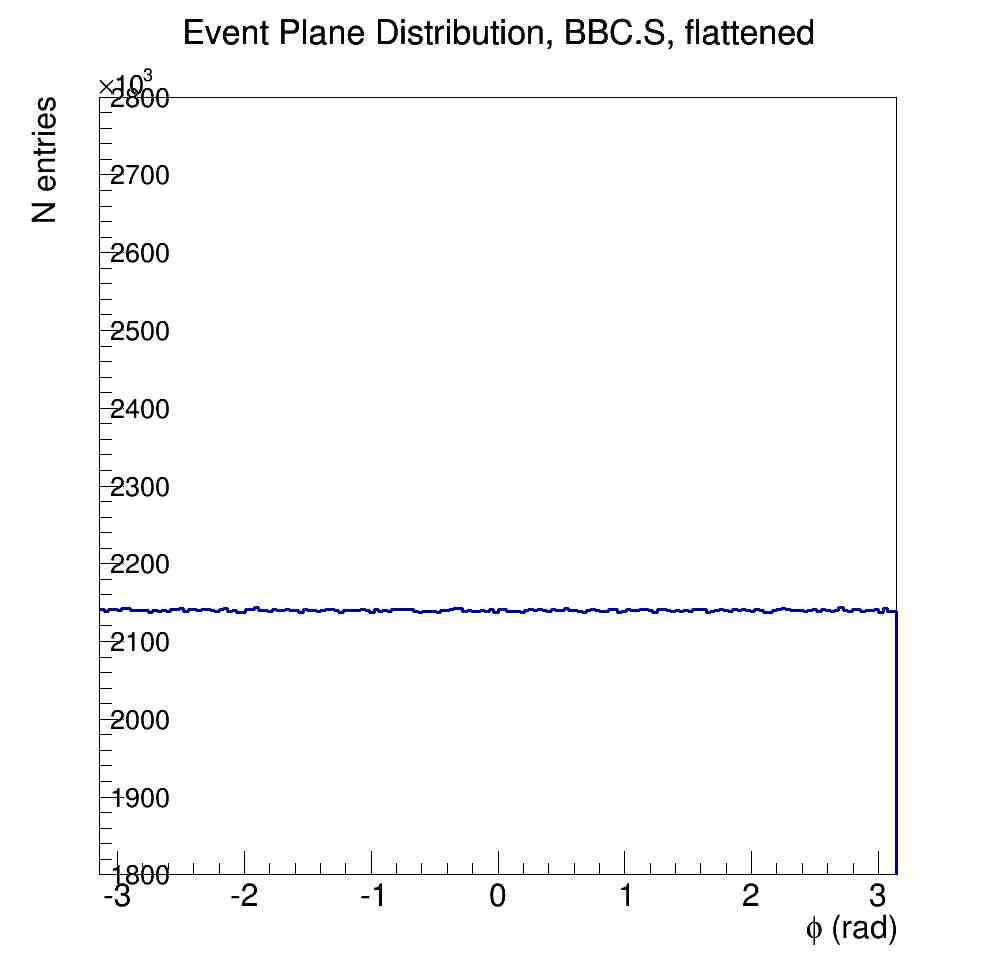
\includegraphics[width=1\textwidth]{EPflattening/flatbbcs.jpg}
    \end{subfigure}
    \begin{subfigure}[p]{0.4\textwidth}
    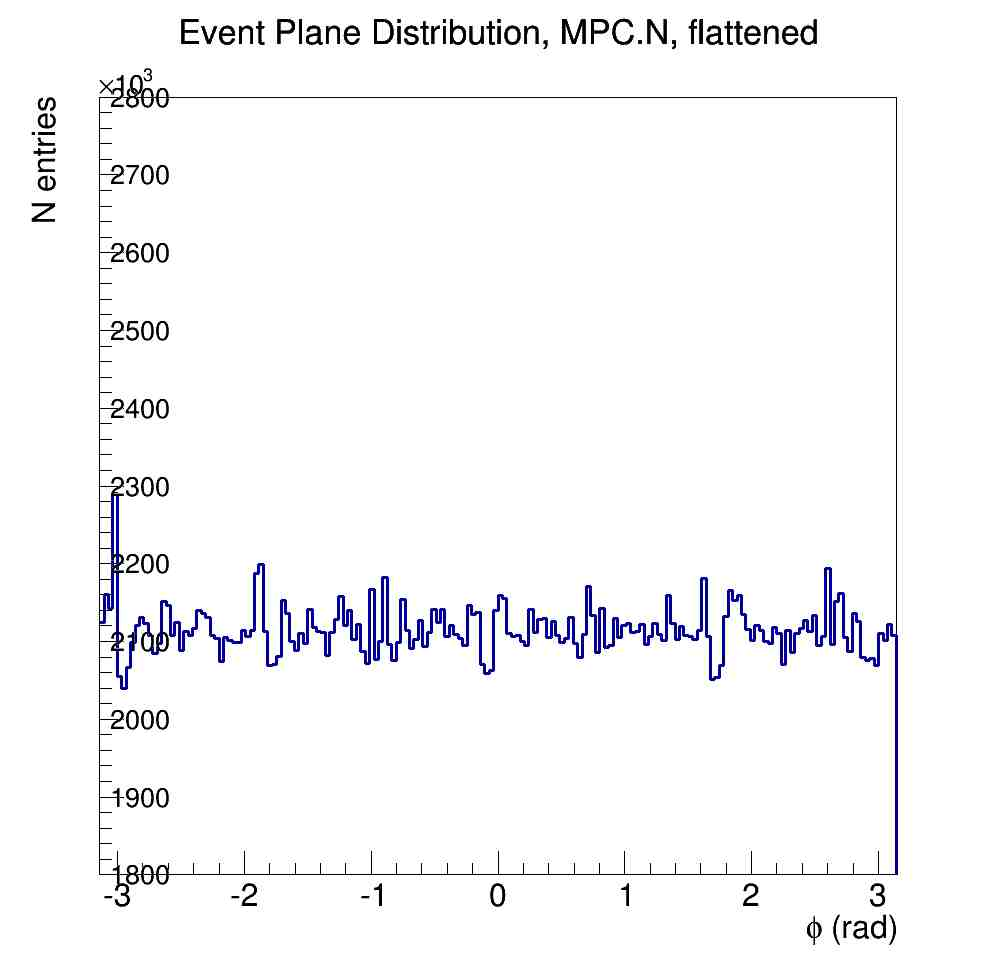
\includegraphics[width=1\textwidth]{EPflattening/flatmpcn.jpg}
    \end{subfigure}
    \begin{subfigure}[p]{0.4\textwidth}
    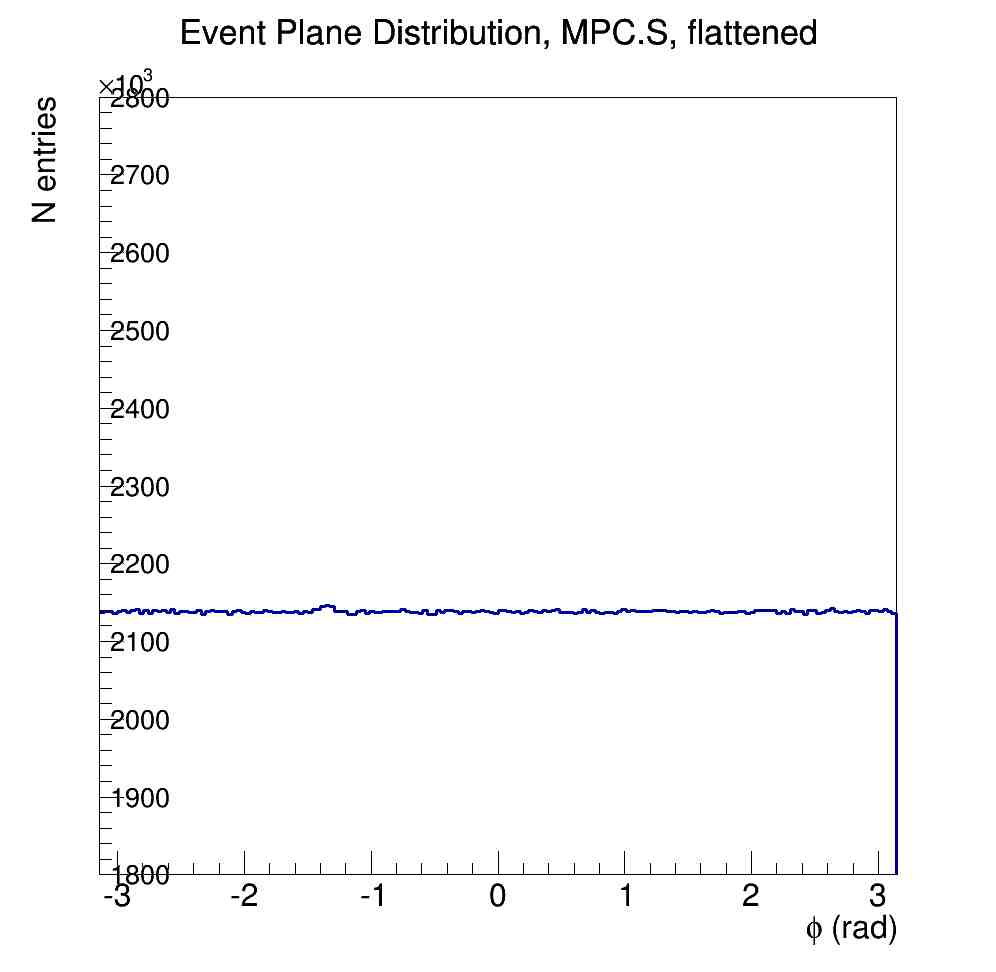
\includegraphics[width=1\textwidth]{EPflattening/flatmpcs.jpg}
    \end{subfigure}
    \begin{subfigure}[p]{0.4\textwidth}
    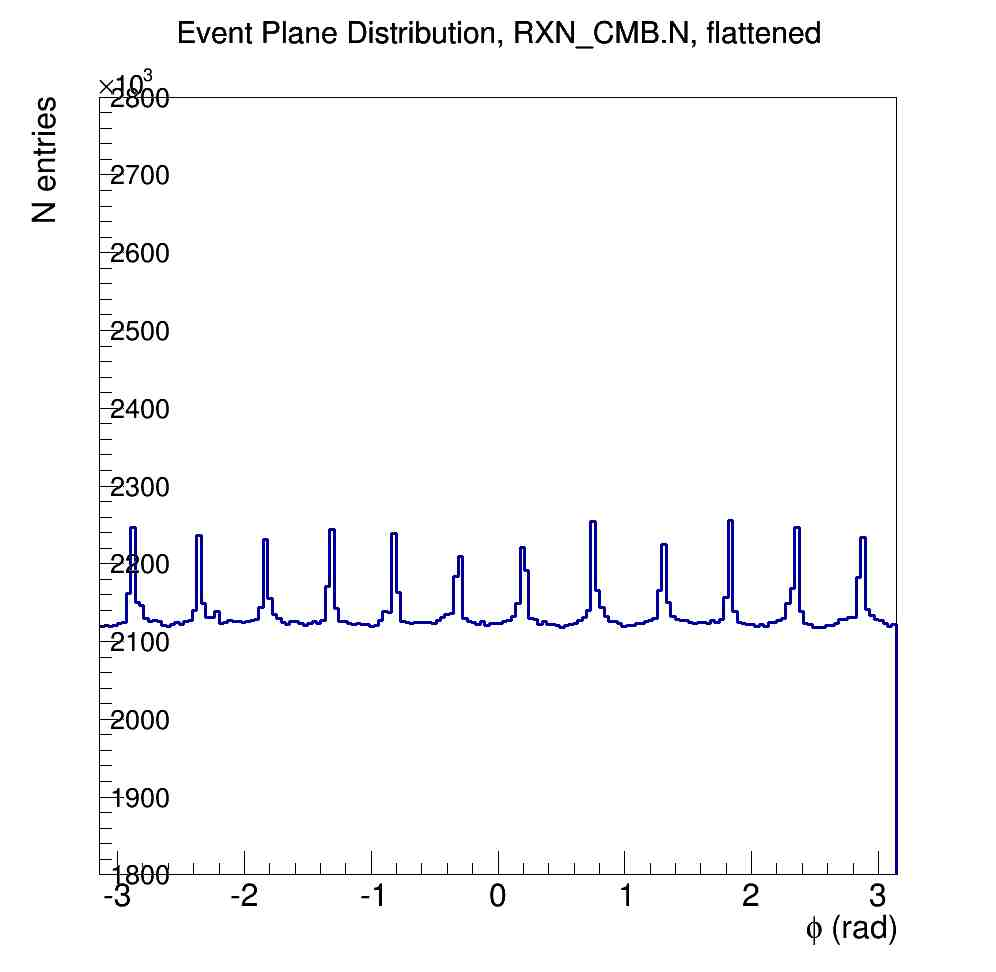
\includegraphics[width=1\textwidth]{EPflattening/flatrxncmbn.jpg}
    \end{subfigure}
    \begin{subfigure}[p]{0.4\textwidth}
    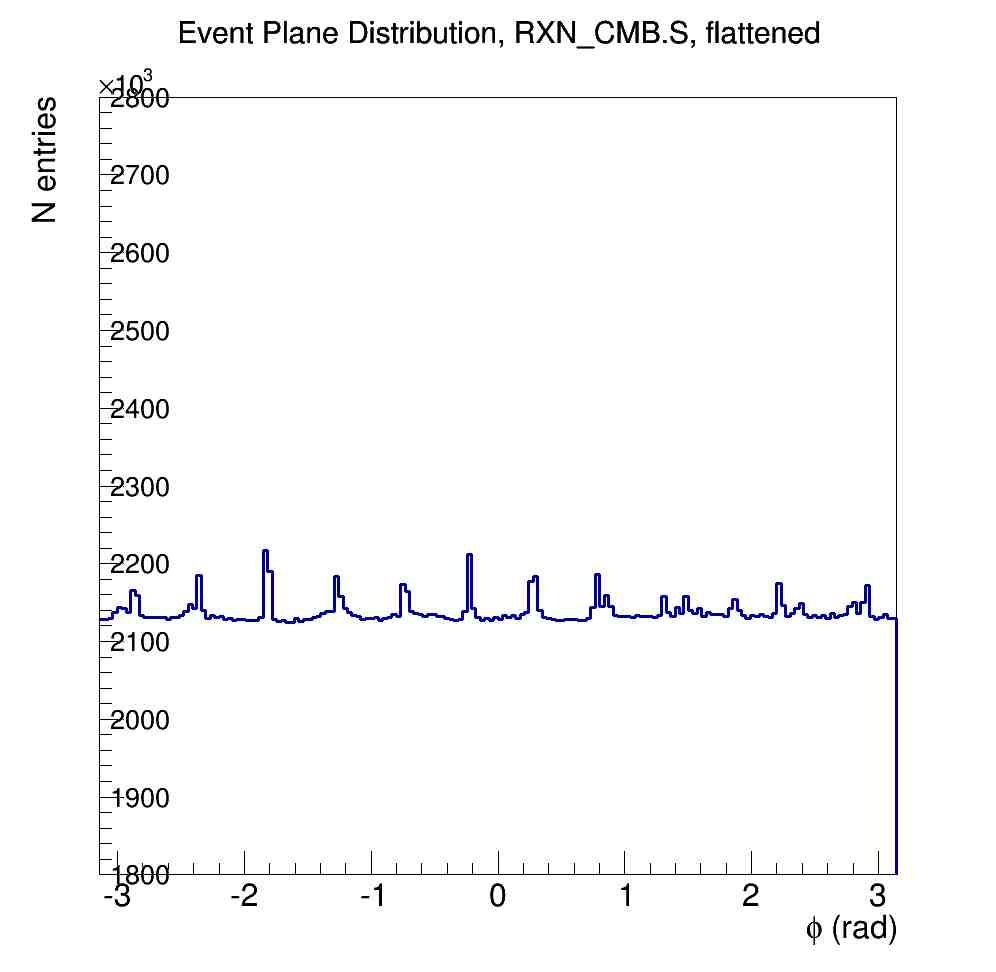
\includegraphics[width=1\textwidth]{EPflattening/flatrxncmbs.jpg}
    \end{subfigure}
    \rule{35em}{0.5pt}
  \caption[Flattened event plane distributions in the BBC, MPC, and RXNP]{Flattened event plane distributions in the BBC, MPC, and RXNP. Note that this flattening is significantly better in the ``gold-going'' south arm.}
  \label{fig:evtpln}
\end{figure}

The d+Au system is asymmetric by construction, therefore track multiplicities on the north and south detectors are not the same. Since gold ions have a considerably larger number of nucleons than deuterons, they therefore have higher forward track multiplicity, and their event plane signature in the forward detectors is much stronger. In practice, the north side is the deuteron-going side, and the south side is the gold-going side. This can be seen clearly in Figure \ref{fig:evtpln} where the event plane is much easier to flatten in the south than in the north, regardless of which detector subsystem is chosen.

\section{Event Plane Resolution Correction}
\label{sect:epres}
Since there is a finite track multiplicity, the track distribution is not smooth and continuous across the detectors; rather there is an associated resolution limitation for each measurement made with a specific detector. This resolution limitation affects how well flow anisotropies can be measured, and, because of the nature and shape of various Fourier harmonics, higher harmonics are more strongly affected by resolution limitations since their shape is quickly varying over the azimuthal distribution compared to lower harmonics. Due to this, resolution corrections must be calculated for each harmonic separately. The apparatus makes different measurements of the event plane assuming the shape of specific Fourier harmonics; therefore, the resolution corrections made for each detector are specific to the $n$ of the harmonic. That is to say, the harmonic dependence and detector resolution dependence of the resolution correction are not separable. Additionally, by collision geometry, the ability to determine each correction is dependent on event centrality, implying that these corrections must be made for each centrality bin as well. The measured flow anisotropy decreases as the ability to resolve changes in flow decreases, so this resolution error is corrected by defining some multiplicative scaling such that
\begin{equation}
v_n = \frac{v_n^{A}}{Res(\Psi_n^A)}
\end{equation}
where $v_n^{A}$ is the $n^{th}$ order anisotropic flow coefficient measured with some detector, arbitrarily designated \textit{A}, and $Res(\Psi_n^A)$ is a single valued correction factor for the $v_n$ measurement using a specific detector and a single bin in centrality. Since device resolution is independent of particle species, the calculation of a different correction for each particle flow is not needed. 

The method of determining resolution corrections used for this analysis is called the \textit{Three Subevent Method}. It can be calculated by comparing the event plane measured by one detector with measurements made by two other detectors. For instance, the resolution correction for detector A using the Three Subevent Method with detectors B and C can be defined as \citep{PhysRevC.58.1671}

%Specifically, we take a measurement of the event plane made by the detector whose resolution we would like to correct (say, detector A) and subtract a measurement of the same event plane made by another detector (detector B) take the cosine of two times that difference, i.e. $\langle cos(2k[\Psi^{A}-\Psi^{B}])\rangle$. This $cos (2 *\Delta \Psi)$ is chosen here since we are calculating the resolution correction for the 2nd harmonic. This gives us one approximation of the resolution correction but it is conceptually still dependent on the resolution limitations of detector B. We then take another approximation of the correction using a different detector (C) so we have the resolution limitation of detector A as measured by B and C. Then we can try to remove the dependence on B and C's resolution by dividing by another resolution approximation made using B and C's measurement. 
%----------------------------------------------------------------------------------------
\begin{equation}
\label{eqn3se}
Res\{n \Psi_n^{A}\} = \sqrt{\frac{\langle cos(n[\Psi_n^{A}-\Psi_n^{B}])\rangle \langle cos(n[\Psi_n^{A}-\Psi_n^{C}])\rangle}{\langle cos(n[\Psi_n^{B}-\Psi_n^{C}])\rangle}}
\end{equation} 
where $\Psi_n^X$ is the event plane as measured with detector X using the n$^{th}$ Fourier harmonic.
\pagebreak
\pagebreak
